\usepackage[T1]{fontenc}
\usepackage{pslatex}
 \usepackage[pdftex]{color}  
 \usepackage[pdftex]{graphicx}     
\usepackage{verbatim}
\usepackage{xcolor}
\usepackage{paralist}
\usepackage{tagging}

\usepackage[colorlinks=true,urlcolor=red]{hyperref}
\setlength{\topmargin}{-0.5in}                  % topmargin now at 1in
\setlength{\textheight}{9.5in}                  % body of text = 9.5in
\setlength{\oddsidemargin}{0in}                 % left margin = 1.0in on odd-numbered pages
\setlength{\evensidemargin}{0in}                % left margin = 1.0in on even-numbered pages 
\setlength{\textwidth}{6.5in}                   % width of text line.
\setlength{\parindent}{0.0in}
\newcommand{\code}{\texttt}

\usepackage{listings}
\lstset{%
	language=Java,
	basicstyle=\footnotesize\ttfamily,
	numbers=left,
	numberstyle=\tiny,        
	xleftmargin=17pt,
        	xrightmargin=5pt,
	frame=single,
	breaklines=true,
	moredelim=\item \item [is][\color{red}]{@}{@}
}

\begin{document}

\definecolor{aquamarine}{rgb}{0,0,0.7}
\definecolor{blue}{rgb}{0,0,0.7}
\definecolor{red}{rgb}{1,0,0}

%
\vspace{0.2in}
\begin{center}
        {\large  %MACQUARIE UNIVERSITY\\
%\medskip
\includegraphics[scale=0.3]{../../logo.png}\\
\medskip
        {\it  Faculty of Science and Engineering\\}
        \vspace{0.2in}
         {\bf COMP125 Fundamentals of Computer Science\\
        Workshop Week 11\\}}
\end{center}
\vspace{0.3in}
%

%\renewcommand{\labelenumi}{\arabic{enumi}.}
\renewcommand{\labelenumi}{\alph{enumi}.}
 
\section* {Learning outcomes}

By the end of this session, you will have learnt about linked lists. 

%\begin{center}
%\fbox{
%\begin{minipage}{0.8\textwidth}
%Import project from \texttt{recursionWorkshopTemplate.zip}. 
%\end{minipage}
%}
%\end{center}

\section*{Questions}
\begin{questions}

\question Represent, both as a logical diagram, and a memory diagram, the state of a linked list containing the following items (in the order of appearance in the list),

\begin{enumerate}
\item "going"
\item "on"
\item "tangents"
\item "is"
\item "not"
\item "normal"	

\begin{solution}
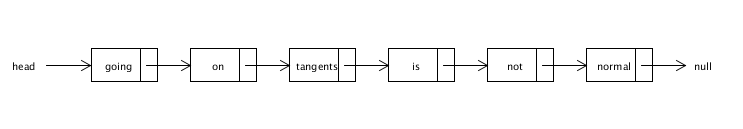
\includegraphics[scale=0.5]{logical.png}	
\vskip 1cm
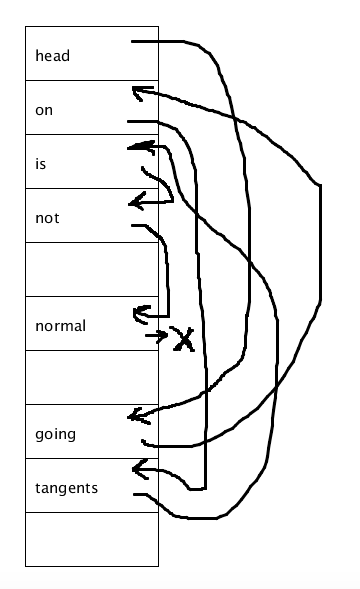
\includegraphics[scale=0.5]{memory.png}
\end{solution}

\end{enumerate}

\question
A \texttt{LinkedList} is a resizable set of objects such that each item links to the next item. If you don't parameterise an \texttt{LinkedList}, it can hold a variety of objects. That is, each item of the \texttt{LinkedList} can be of a different class.

A parameter-less \texttt{LinkedList} is created as -

\begin{lstlisting}
    LinkedList list = new LinkedList();
\end{lstlisting}
where \texttt{list} is the \texttt{LinkedList} object.

You can parameterize an \texttt{LinkedList} so that it stores objects of a specific class. A parameterized \texttt{LinkedList} is created as -

\begin{lstlisting}
    LinkedList<ClassType> list = new LinkedList<ClassType>();
\end{lstlisting}

where \texttt{list} is the \texttt{LinkedList} object.

\newpage

For example,

\begin{lstlisting}
    LinkedList<String> list = new LinkedList<String>();
\end{lstlisting}

can only hold \texttt{String} objects.

A subset of methods (the important ones) applicable to an \texttt{LinkedList} object is given below -

\begin{itemize}
\item \texttt{int size()}: returns the number of items in the list
\item \texttt{Object get(int index)}: returns the \texttt{Object} at the specified index, if any; and \texttt{null} otherwise.
\item \texttt{add(Object obj)}: adds the specified \texttt{Object} to the end of the list and returns \texttt{true}, if it can; and \texttt{false} otherwise.
\item \texttt{add(int idx, Object obj)}: adds the specified \texttt{Object} at given index. Shifts all items at index \texttt{idx} onwards to the right.
\item \texttt{contains(Object obj)}: returns \texttt{true} if the specified exists, and \texttt{false} otherwise.
\item \texttt{indexOf(Object obj)}: returns the index of the specified \texttt{Object} if it exists, and -1 otherwise.
\item \texttt{remove(Object obj)}: removes the specified \texttt{Object} to the list and returns \texttt{true}, if it can; and \texttt{false} otherwise.
\item \texttt{set(int index, Object obj)}: updates the item at given index ot the object passed. Returns the item that the new object has replaced.
\end{itemize}

Write a piece of code that performs the following operations in the given order -

\begin{enumerate}
	\item Create a linked list of integers
	\item Add items (in that order) to the end of the list: 30, 70, 40, 80, 20, 100, 60
	\item Update the list so that each item becomes twice of its current value
	\item Calculate and store the highest value in the list in a variable \texttt{max}
\end{enumerate}

\begin{solution}
	\begin{lstlisting}
LinkedList<Integer> list = new LinkedList<Integer>();
list.add(30);
list.add(70);
list.add(40);
list.add(80);
list.add(20);
list.add(100);
list.add(60);
for(int i=0; i < list.size(); i++)
	list.set(i, list.get(i) * 2);
int max = list.get(0);
for(Integer item: list)
	if(item > list)
		max = item;
	\end{lstlisting}
\end{solution}

\question (Assessed task) Write a method \texttt{countPositives} that when passed an \texttt{LinkedList} of \texttt{Double} objects, returns the number of positive items in the \texttt{LinkedList}. The method should return 0 if the list is \texttt{null} or empty.

\begin{lstlisting}
	public static int countPositives(LinkedList <Double> list)
\end{lstlisting}

\begin{solution}
\begin{lstlisting}
public static int countPositives(LinkedList <Double> list) {
		if(list == null || list.size() == 0) 
			return 0;
		int result = 0;
		for(Double item: list)
			if(item > 0)
				result++;
		return result;
	}	
\end{lstlisting}	
\end{solution}


\question (Assessed task) Write a method \texttt{countMatches} that when passed an \texttt{LinkedList} of \texttt{String} objects and a String \texttt{target}, returns the number of items in the list that contains \texttt{target}. The method should return 0 if the list is \texttt{null} or empty. For example, if \texttt{list = ["thereby", "they", "proved", "the", "other", "guy", "was", "the", "father"]} and \texttt{target = "the"}, the method should return 6, as there are six Strings containing \texttt{"the"}.

\begin{lstlisting}
	public static int countMatches(LinkedList<String> list, String target)
\end{lstlisting}

\begin{solution}
\begin{lstlisting}
	public static int countMatches(LinkedList<String> list, String target) {
		if(list == null || list.size() == 0) 
			return 0;
		int result = 0;
		for(String item: list)
			if(item.contains(target))			
				result++;
		return result;
	}	
\end{lstlisting}	
\end{solution}

\question (Assessed Task) Add a method \texttt{count} that when passed an \texttt{LinkedList<Integer> list}, returns the number of prime numbers in \texttt{list}.

\begin{lstlisting}
	public static int countPrimes(LinkedList<Integer> list)
\end{lstlisting}

\begin{solution}
\begin{lstlisting}
public static int countPrimes(LinkedList<Integer> list) {
	if(list == null)
		return 0;
	int result = 0;
	for(Integer item: list)
		if(isPrime(item))
			result++;
	return result;
}

public static boolean isPrime(int n) {
	if(n < 2)
		return false;
	for(int i=2; i*i < n; i++)
		if(n%i == 0)
			return false;
	return true;
}
\end{lstlisting}
\end{solution}

\question (Voluntary assessed task) Write a method that when passed a \texttt{LinkedList} of integers, returns a number constructed with the first digit of each item of the list. The method should return 0 if the list is \texttt{null} or empty. For example, if the list is [15, 673, 8914], the method returns the number 168.

\begin{solution}
\begin{lstlisting}
public static int getFirstDigitNumber(LinkedList <Character> list) {
	if(list == null) 
		return null;
	int result = 0;
	for(Integer item: list)
		result = result*10 + firstDigit(item);
	return result;
}	

public static int firstDigit(int n) {
	if(n == 0)
		return 0;
		
	if(n < 1)
		n*=-1;
	
	while(n > 10) {
		n/=10;
	}
	return n;
}
\end{lstlisting}	
\end{solution}


\question (Voluntary assessed task) Write a method \texttt{getPerfectSquares} that when passed a \texttt{LinkedList<Integer> list}, returns a list containing perfect squares (squares of integers) in that list.

\begin{lstlisting}
public static LinkedList<Integer> getPerfectSquares(LinkedList<Integer> list)
\end{lstlisting}

\begin{solution}
\begin{lstlisting}
public static LinkedList<Integer> getPerfectSquares(LinkedList<Integer> list) {	if(list == null)
		return null;

	LinkedList<Integer> result = new LinkedList<Integer>();
	for(Integer item: list) {
		double root = Math.sqrt(item * 1.0);
		if((int)root * root == item)
			result.add(item);
	}
	return result;
}
\end{lstlisting}
\end{solution}
\end{questions}
	
\end{document}
